\subsection {Autómata finitos}  
Según \cite{[PINOCHO]} un autómata finito (máquina de estados finitos), es un modelo computacional que realiza cómputos en forma automática sobre una entrada para producir una salida.\\
\hspace*{1cm}Este modelo está conformado por un alfabeto, un conjunto de estados y un conjunto de transiciones entre dichos estados. Su funcionamiento se basa en una función de transición, que recibe a partir de un estado inicial una cadena de símbolos pertenecientes al alfabeto (la entrada), y que va leyendo dicha cadena a medida que el autómata se desplaza de un estado a otro, para finalmente detenerse en un estado final o de aceptación, que representa la salida.\\
\hspace*{1cm}La finalidad de los autómatas finitos es la de reconocer lenguajes regulares. Formalmente, un autómata finito es una 5-tupla $<Q, \Sigma, q0, \delta, F>$ donde:
    \begin{itemize}
        \item \textbf{$Q$} es un conjunto finito de estados.
        \item \textbf{$\Sigma$} es un alfabeto finito de símbolos.
        \item \textbf{$q0$} es el estado inicial en Q.
        \item \textbf{$\delta$} es la relación de transiciones de la forma $<qi,x,qj>$ con $qi$ y $qj$ como estados de $Q$ y $x$, símbolo de $\Sigma$ ó puede ser también la cadena vacía.
        \item \textbf{$F$} es el conjunto de estados finales o de aceptación y (evidentemente) subconjunto de $Q$.
    \end{itemize}
    
%\hspace*{1cm}Los autómatas que se abarcara en este tema serán autómatas finitos deterministas y los autómatas finitos no deterministas.\\

\subsubsection {Autómatas finitos deterministas}  
Según \cite{[PINOCHO2]} un autómata finito determinista (AFD) es un autómata finito que además es un sistema determinista; es decir, para cada estado $q \in Q$ en que se encuentre el autómata, y con cualquier símbolo $\alpha \in \Sigma$ del alfabeto leído, existe siempre a lo más una transición posible $\delta(q,a)$. En la figura \ref{fig:AFN_CONVERTIDO.png} se puede apreciar un ejemplo de un AFD que consta de los elementos mencionados en la lista anterior:

\begin{itemize}
\item \textbf{$Q$}: (q0,q1,q2).
\item \textbf{$\Sigma$}: (a,b).
\item \textbf{$q0$}: (q0).
\item \textbf{$\delta$}: es la relación de transiciones que se muestran en la tabla \ref{table:AFN_CONVERTIDO}.
\item \textbf{$F$}: (q2).
\end{itemize}

\begin{table}[hbtp]
\centering
   \caption{Ejemplo de transiciones de un AFD.}
   \begin{tabular}{ | l | l | l |}
   \hline
     \rowcolor[gray]{0.5}
          &   a  &  b   \\ \hline
       q0 &  q1  & q0   \\ \hline   
       q1 &  q1  & q2   \\ \hline
      *q2 &  q1  & q0   \\ \hline
   \end{tabular}
   \label{table:AFN_CONVERTIDO}
\end{table}

    \begin{figure}[hbtp]
        \centering
            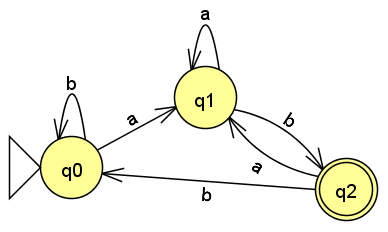
\includegraphics[width=0.5\textwidth]{MarcoTeorico/Imagenes/AFN_CONVERTIDO.png}
            \caption{Ejemplo de autómata finito determinista.}     
            \label{fig:AFN_CONVERTIDO.png}
    \end{figure} 

\hspace*{1cm}El autómata en cuestión acepta solamente las cadenas de símbolos que terminen con $ab$, una vez que ya no existen más caracteres y éste cae en el estado $q2$ (aquél que está en doble círculo) significa que es una cadena válida para el autómata.\\
\hspace*{1cm}En un AFD no pueden darse ninguno de estos dos casos:
    \begin{itemize}
        \item Que existan dos transiciones del tipo $\delta(q,a)=q1$ y $\delta(q,a)=q2$, siendo $q1 \neq q2$;
        \item Que existan transiciones del tipo $\delta(q,\epsilon)$, salvo que q sea un estado final, sin transiciones hacia otros estados.
    \end{itemize}    
\subsubsection {Autómatas finitos no deterministas}      
Según \cite{[PINOCHO3]} un autómata finito no determinista (AFND) es aquél que, a diferencia de los autómatas finitos deterministas, posee al menos un estado $ q \in Q$, tal que para un símbolo $\alpha \in \Sigma$ del alfabeto, existe más de una transición $\delta(q,a)$ posible. Haciendo la analogía con los AFDs, en un AFND puede darse cualquiera de estos dos casos:
    \begin{itemize}
        \item Que existan transiciones del tipo $\delta(q,a)=q1$ y $\delta(q,a)=q2$, siendo $q1 \neq q2$;
        \item Que existan transiciones del tipo $\delta(q,\epsilon)$, siendo q un estado no-final, o bien un estado final pero con transiciones hacia otros estados.
        \item Cuando se cumple el segundo caso, se dice que el autómata es un autómata finito no determinista con transiciones vacías o transiciones $\epsilon$ (abreviado AFND-$\epsilon$). Estas transiciones permiten al autómata cambiar de estado sin procesar ningún símbolo de entrada.
        \item También hacen transiciones $\epsilon$ que son aquellas donde se mueve a otro estado sin hacer nada, siempre y cuando el estado actual lo indique.
    \end{itemize}
\hspace*{1cm}Haciendo un ejemplo con el autómata de la figura \ref{fig:AFN_CONVERTIDO.png} se puede observar que se puede hacer un AFND con la misma cadena de aceptación:

    \begin{figure}[hbtp]
        \centering
            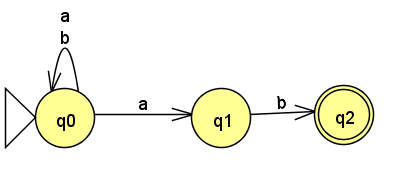
\includegraphics[width=0.5\textwidth]{MarcoTeorico/Imagenes/AFN.png}
            \caption{Ejemplo de autómata finito no determinista.}     
            \label{fig:AFN.png}
    \end{figure} 
    
\hspace*{1cm}Como se puede observar en la figura \ref{fig:AFN.png} tiene una menor cantidad de transiciones, como se puede ver en la tabla \ref{table:AFN} el estado $q0$ produce 2 estados en la transición $a$, una que lleva al estado $q1$ y otra que lleva nuevamente al estado $q0$, es este momento en el que se hacen 2 procesos por separado, cada uno siguiendo un distinto estado así sucesivamente hasta que termine la cadena.

\begin{table}[hbtp]
\centering
   \caption{Ejemplo de transiciones de un AFND.}
   \begin{tabular}{ | l | l | l |}
   \hline
     \rowcolor[gray]{0.5}
          &   a     &  b   \\ \hline
       q0 &  q0,q1  & q0   \\ \hline   
       q1 &         & q2   \\ \hline
      *q2 &         &      \\ \hline
   \end{tabular}
   \label{table:AFN}
\end{table}

\hspace*{1cm}Como se menciona anteriormente, las transiciones $\epsilon$ son, de acuerdo a \cite{[PINOCHO4]}, transiciones que permiten ir a otro estado sin necesidad de un símbolo. La figura \ref{table:EjemploAFND} muestra un autómata que acepta la expresión regular ($0*1*2*$):

 \begin{itemize}
\item \textbf{$Q$}: (q0,q1,q2).
\item \textbf{$\Sigma$}: (0,1,2).
\item \textbf{$q0$}: (q0).
\item \textbf{$\delta$}: es la relación de transiciones que se muestran en la tabla \ref{table:EjemploAFND}.
\item \textbf{$F$}: (q2).
\end{itemize}

 \begin{table}[hbtp]
\centering
   \caption{Ejemplo de AFND con transición $\epsilon$.}
   \begin{tabular}{ | l | l | l | l | l |}
   \hline
     \rowcolor[gray]{0.5}
          &  0  &  1  &  2  & $\epsilon$   \\ \hline
       q0 & q0  &     &     & q1           \\ \hline   
       q1 &     & q1  &     & q2           \\ \hline
      *q2 &     &     & q2  &              \\ \hline
   \end{tabular}
   \label{table:EjemploAFND}
\end{table}

 \begin{figure}[hbtp]
    \centering
        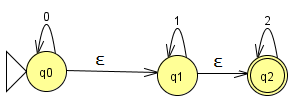
\includegraphics[width=0.5\textwidth]{MarcoTeorico/Imagenes/aufnd_b.png}
        \caption{Ejemplo de AFND con transición $\epsilon$.}     
        \label{fig:aufnd.png}
\end{figure} 

\hspace*{1cm}Como se puede observar en este ejemplo, la transición $\epsilon$ permite saltar de un estado a otro sin usar un símbolo; en caso de que el siguiente estado no posea ninguna transición con el símbolo actual puede tomar (en caso de que tenga) la transición $\epsilon$ actuando como un sustituto. También se puede dar el caso de que exista una transición $\epsilon$ y una transición con el símbolo actual. En este caso se generan 2 procesos en paralelo para satisfacer ambas transiciones. En el siguiente ejemplo se puede explicar lo mencionado anteriormente:

 \begin{itemize}
\item \textbf{$Q$}: (q0,q1,q2,q3).
\item \textbf{$\Sigma$}: (a,b).
\item \textbf{$q0$}: (q0).
\item \textbf{$\delta$}: es la relación de transiciones que se muestran en la tabla \ref{table:EjemploAFND2}.
\item \textbf{$F$}: (q2).
\end{itemize}

\begin{table}[hbtp]
\centering
   \caption{Segundo ejemplo de un AFND con transición $\epsilon$.}
   \begin{tabular}{ | l | l | l | l |}
   \hline
     \rowcolor[gray]{0.5}
          & a &  b     & $\epsilon$   \\ \hline
       q0 &   & q1,q3  & q0          \\ \hline   
       q1 &   & q2     &             \\ \hline  
      *q2 &   &        &             \\ \hline  
       q3 &   &        & q2          \\ \hline  
   \end{tabular}
   \label{table:EjemploAFND2}
\end{table}

 \begin{figure}[hbtp]
    \centering
        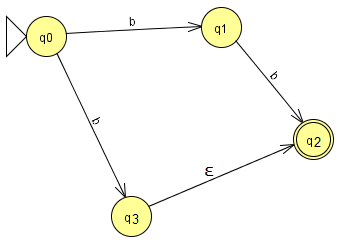
\includegraphics[width=0.5\textwidth]{MarcoTeorico/Imagenes/AFN2_b.png}
        \caption{Segundo ejemplo de AFND con transición $\epsilon$.}     
        \label{fig:AFN2.png}
\end{figure} 

\hspace*{1cm}En este ejemplo se puede observar que este autómata acepta solamente las cadenas $b$ y $bb$. En el estado inicial la transición $b$ lleva a dos estados distintos, en ese momento se tomarán en cuenta los 2 estados $q1$ y $q3$ donde el estado $q1$ podrá llegar al estado de aceptación $q2$ si encuentra otra cadena $b$ mientras que el estado $q3$ podrá llegar a su estado de aceptación si no existe otra cadena (que se interpreta con la transición $\epsilon$).\\